\documentclass[a4paper,10pt,twoside]{article}
%%%%%%%%%%% Packages %%%%%%%%%%
\usepackage[margin=1in]{geometry}
\usepackage{amsmath, amssymb,mathtools}
\usepackage{fancyhdr}
\usepackage{sectsty}
\usepackage{graphicx,wrapfig}
\usepackage{enumitem}
\usepackage{float}
\usepackage{braket}
\usepackage{bbm}
\usepackage{tikz,calc}
\usepackage{amsthm}


%%%%%%%%%%% Macros %%%%%%%%%%
\def \note#1 {\vspace{-1em}\paragraph{\bfseries #1}}
\def \dd {{\rm d}}
\def \id {{\mathbbm{1}}}
\def \order {\mathcal{O}}
\def\bquad{\mkern-18mu}
\DeclareMathOperator{\trace}{tr}
\DeclareMathOperator{\spanset}{span}

%%%%%%%%%%% Tikz Definitions %%%%%%%%%%
\usetikzlibrary{shapes, arrows,positioning,fit}
\tikzstyle{plain} = [draw,thick,circle,inner sep=0,minimum size=0.5cm,font=\footnotesize]
\tikzstyle{mps} = [draw,thick,rectangle,rounded corners=.1cm,inner sep=0,minimum size=0.5cm]
\tikzstyle{mpo} = [draw,thick,circle,inner sep=0,minimum size=0.5cm]
\tikzstyle{index} = [-,thick,font=\footnotesize]
\tikzstyle{virtual} = [-,thick,dotted,font=\footnotesize]

\def \tu {0.25cm}

%%%%%%%%%%% Formatting %%%%%%%%%%
\pagestyle{fancy}
\renewcommand{\footrulewidth}{0.5pt}

\fancyhf{}
\lhead{18/05/2017}
\chead{Quantum Information Methods in Many-Body Physics}
\rhead{PH2269}
\lfoot{Giacomo Giudice~~~~giacomo.giudice@mpq.mpg.de}
\rfoot{Page \thepage}

\allsectionsfont{\normalfont\sffamily}

\newtheoremstyle{modern}{3pt}{3pt}{\itshape}{}{\sffamily\bfseries}{}{.5em}{}
\theoremstyle{modern}
\newtheorem{lemma}{Lemma}[section]
\newtheorem{theorem}[lemma]{Theorem}

%%%%%%%%%%% Here Begins Document %%%%%%%%%%
\begin{document}
\title{\vspace{-1cm}\sffamily Homework 5\vspace{-1cm}}
\author{}
\date{}
\maketitle
\thispagestyle{fancy}

\begin{section}{The Toric Code Ground State}
We consider a square lattice, with periodic boundary condition, defining a set of $N$ vertices $+$ and a set of plaquettes $\Box$.
We place spins on the edges, and define the toric code Hamiltonian as
\[
  H = -\sum_{v \in +} A_v - \sum_{p \in \Box} B_p ,
\]
where the $A_v$ act with the Pauli operator $Z$ on the edges adjacent a vertex $v$, while $B_v$ act with $X$ on the edges of a plaquette $p$.
Show that all terms in $H$ commute, i.e. $[A_v,B_p] = 0,\ \forall v \in + , \forall p \in \Box$.
We now define the following states
\[
  \ket{\Psi^0} = \prod_{p \in \Box} \frac{1}{\sqrt{2}} \left(\id + B_p\right) \ket{0 0 \dots 0 0}.
\]
What is the action of $A_v$ and $B_p$ on this state? 
Use this to prove  that $\ket{\Psi^0}$ is an eigenstate of $H$.
What is the eigenvalue?
Argue that this state is a ground state of the toric code.

We will now see how to interpret the state $\ket{\Psi^0}$.
Convince yourself that we can rewrite the ground state as
\[
   \ket{\Psi^0} = \frac{1}{2^{N/2}}\left( \id + \sum_{n=1}^N \sum_{p_1 \neq \dots \neq p_n} \!\! B_{p_1}\dots B_{p_n}\right) \ket{0 0 \dots 0 0} .
\]
where the second sum runs over all possible combinations of $n$ \emph{distinct} plaquettes.
Now consider a subset of adjacent plaquettes. 
Using the notation introduced in the lecture, show that the action of their $B_v$ on the vacuum state gives a closed loop.
Can you see why we say that the ground state is the sum over all possible loop configurations?

\begin{wrapfigure}{r}{0.25\textwidth}
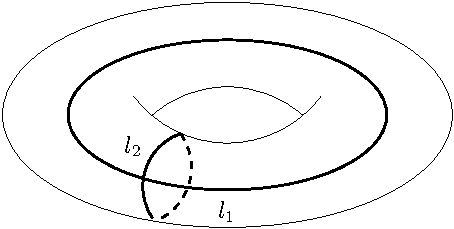
\includegraphics[width=0.25\textwidth]{img/torus-loops}
\end{wrapfigure}

On the torus, there are then additional ground states, $ \ket{\Psi_{ij}^0} = \hat{X}_1^i \hat{X}_2^j \ket{\Psi^0}$, with $ i,j = 0,1$.
The operators $\hat{X}_{1,2}$ flip all the spins along the paths $l_{1,2}$, as shown in the figure.
Show that this is equivalent to
\[
  \ket{\Psi_{ij}^0} = \frac{1}{\sqrt{\rm norm}}\sum_{\mathclap{{\rm loop} \left| \substack{\#_1 = i \\ \#_2 = j } \right. }}  \ \ket{\rm loop} .
\]
Where $\#_1$($ \#_2$) count the number of horizontal (vertical) crossings, modulo 2.
Argue why $\#_{1,2}$ do not depend on the location of the cut.
Show that these $\ket{\Psi^0_{ij}}$ are  ground states of the toric code Hamiltonian and that they are orthogonal between each other.
\end{section}

\begin{section}{Elementary Excitations}
\begin{wrapfigure}{r}{0.5\textwidth}
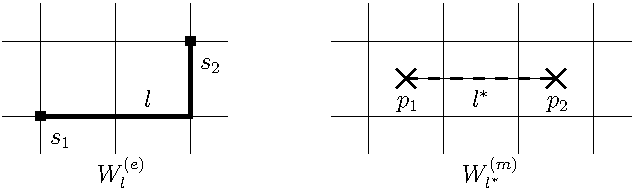
\includegraphics[width=0.5\textwidth]{img/toric-excite}
\end{wrapfigure}
Referring to the figure, let the electric and magnetic path operators be
\[ 
  W_l^{(e)} = \prod_{j \in l} X_j, \quad W_{l^*}^{(m)} = \prod_{j \in l^*} Z_j.
\]
How do these operators commute with $A_v$ and $B_p$?
We now define the excited states 
\[
  \ket{\Psi_{s_1,s_2}^{(e)}} =  W_l^{(e)} \ket{\Psi^0}, \quad \ket{\Psi_{p_1,p_2}^{(m)}} =  W_{l^*}^{(m)} \ket{\Psi^0}.
\]
Show that these states are eigenstates of $H$ and have an energy contribution $+4$ relative to the ground state.
As a matter of fact, they are the first excited states.
\note{Note} Notice how the energy contribution does not depend on the length of the path, we say that the charges are \emph{deconfined}.
\end{section}

\begin{section}{Composite Excitations}
At mentioned at the lecture, an electric and a magnetic excitation sitting at a vertex-plaquette pair behave like a composite particle: $\psi = e \times m$. 
What are the self-statistics of this particle? 
\end{section}

\begin{section}{Boundaries and More}
The toric code can be generalized to planar graphs\footnote{Additionally, we should keep the vertices at the edges \emph{open}, i.e. they don't have a corresponding $A_v$ term (this is also called rough boundary conditions). Do you see why?}, since we can still define $A_v$ and $B_p$, while preserving $[A_v,B_p] = 0$.
Predict the number of ground states of the toric code on a square lattice with two holes and periodic boundary conditions.
\begin{figure}[h]
  \centerline{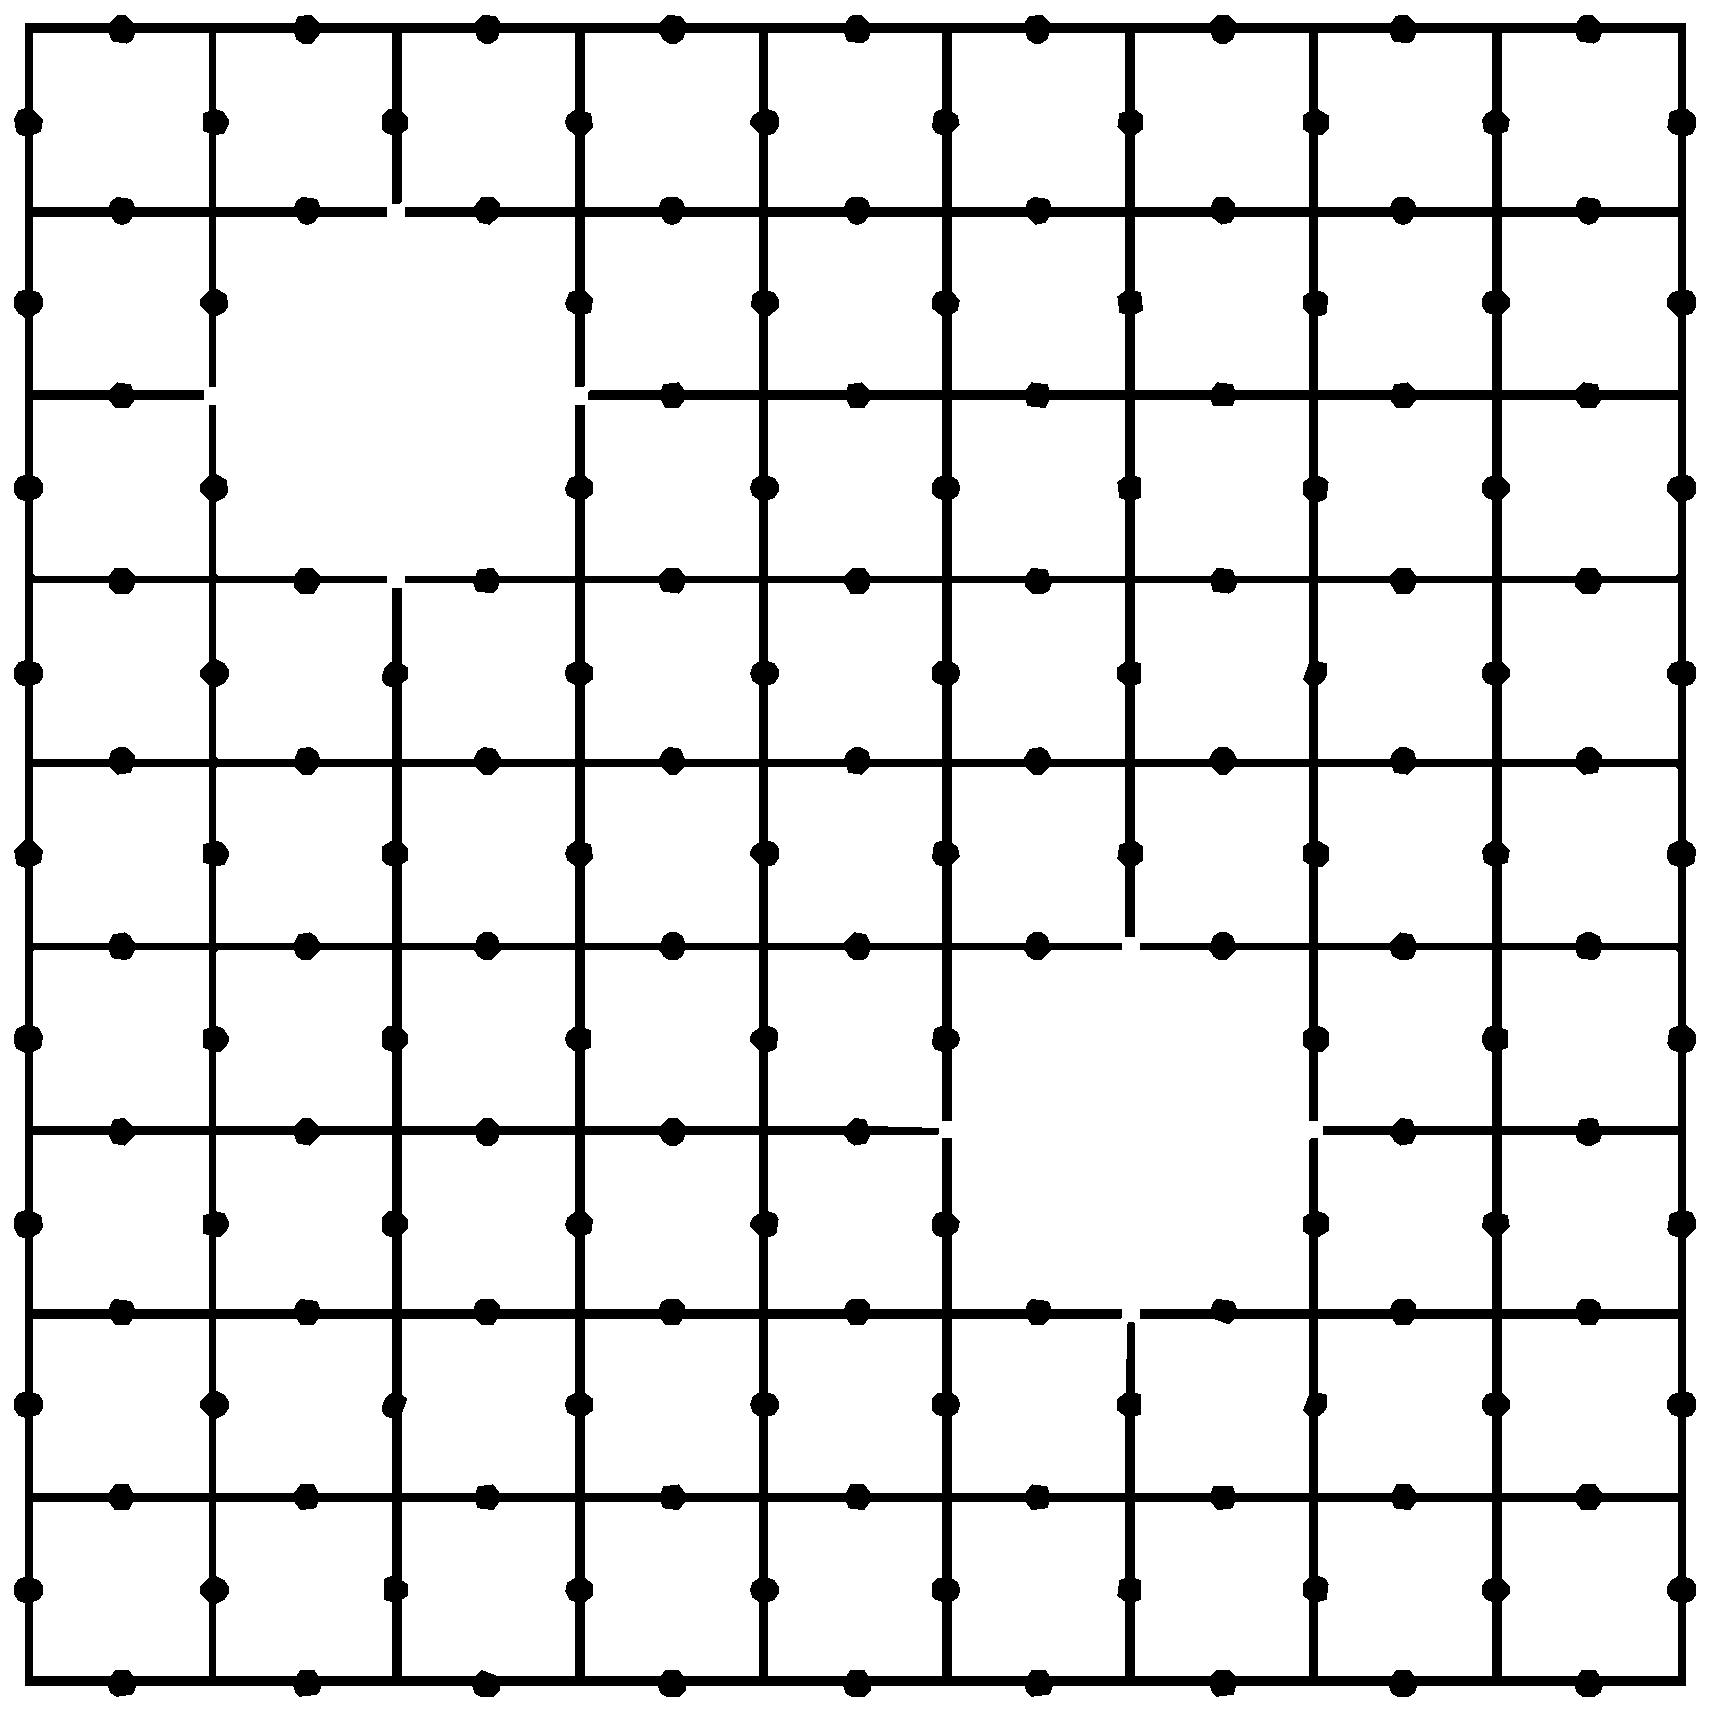
\includegraphics[width=0.25\textwidth]{img/lattice-holes.pdf}}
\end{figure}
\note{Bonus}  Consider the two tori below. On the first torus, a rope is looped through the two holes but does not go around the hole of the torus. On the second, the rope is looped around the hole of the torus. Is it possible to distort the first torus to look like the second? What if the rope does an extra loop around the hole of the torus?
\begin{figure}[h]
  \centerline{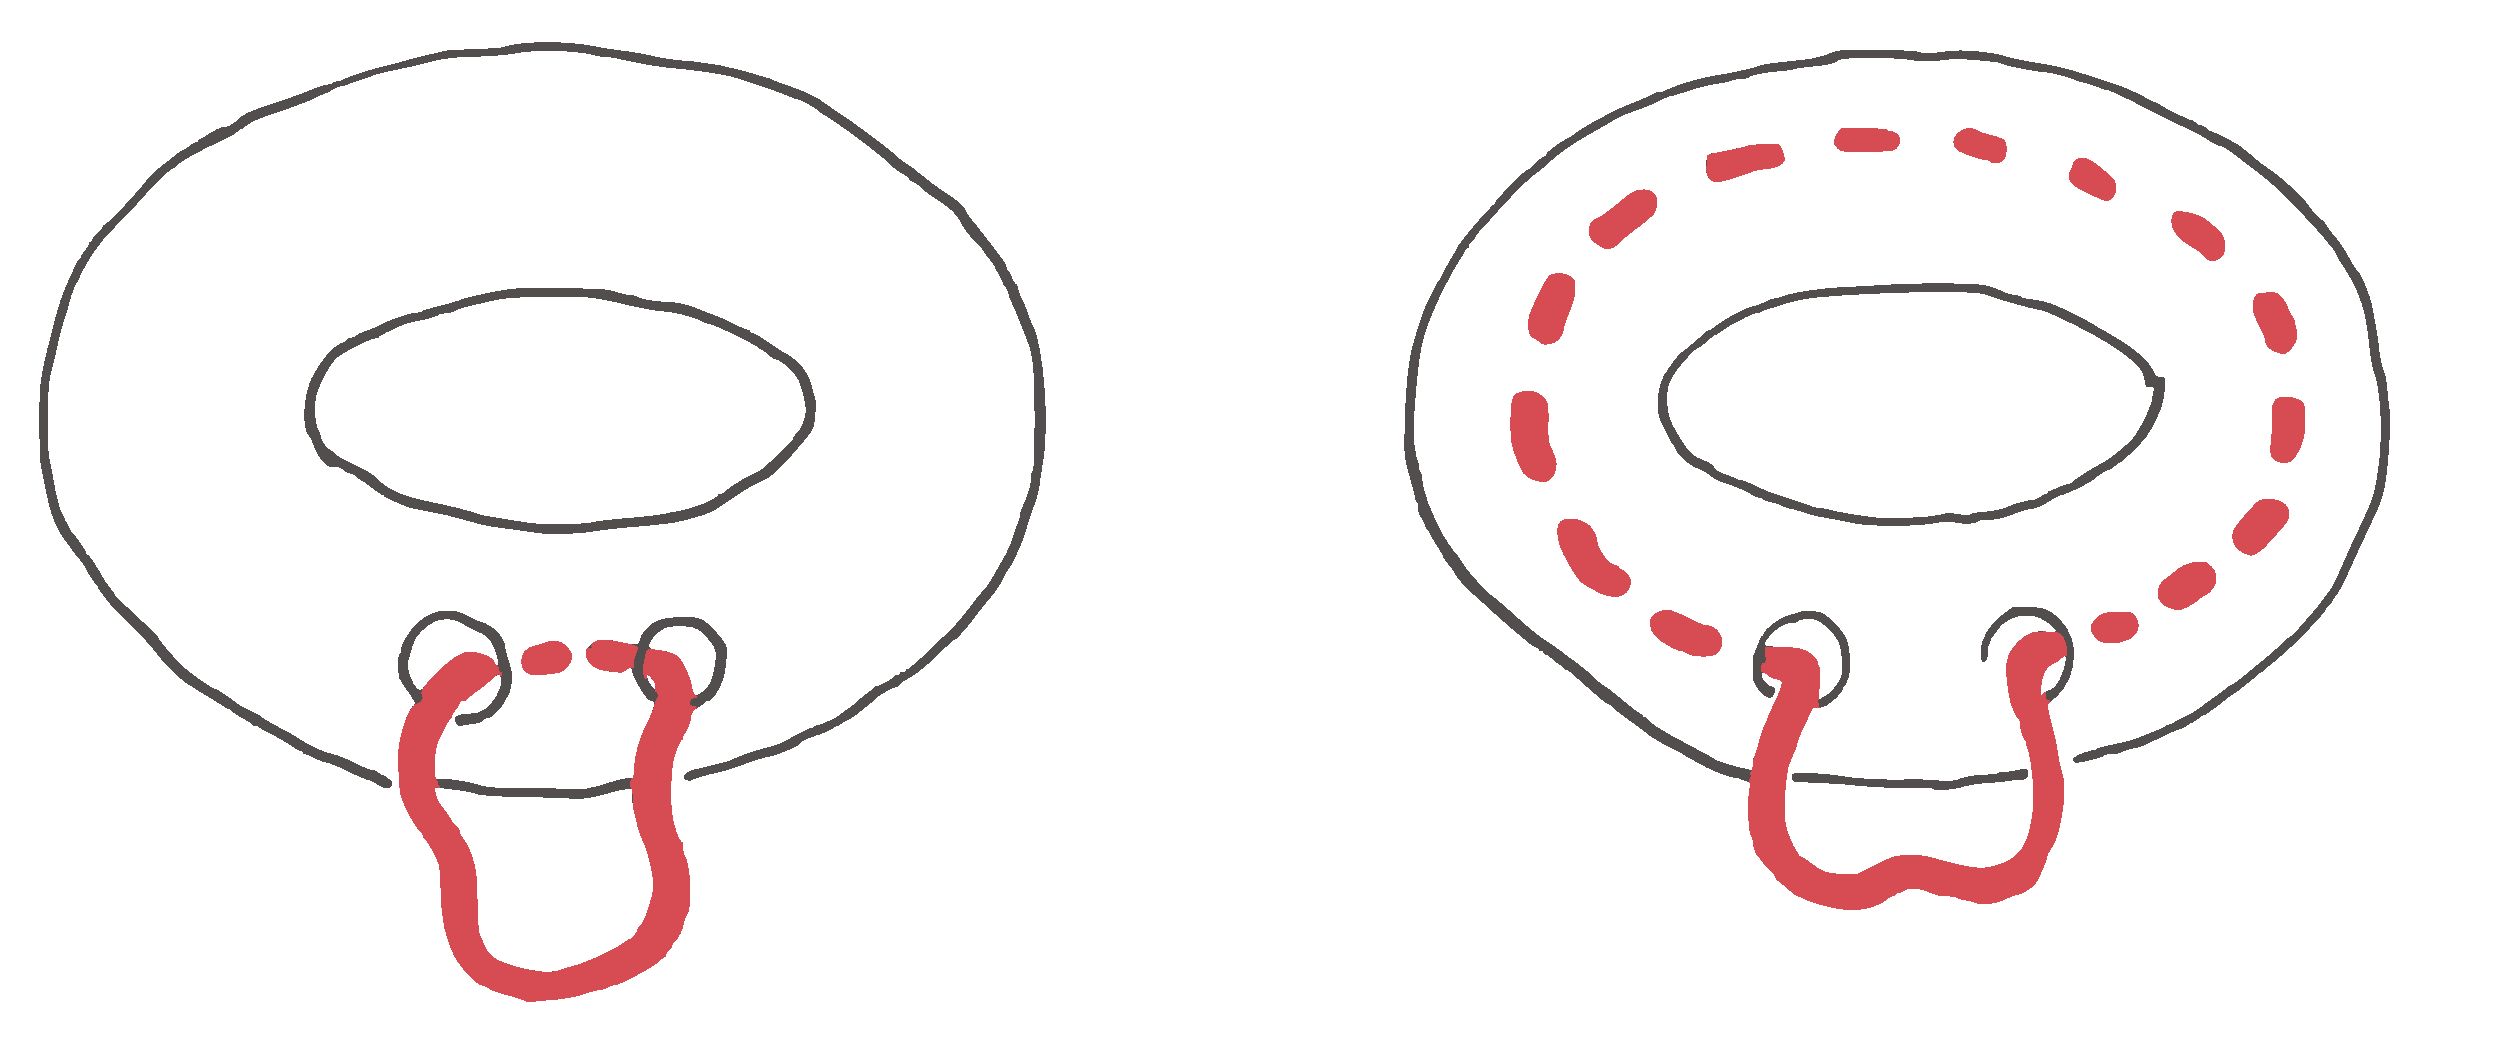
\includegraphics[width=0.4\textwidth]{img/lasso.pdf}}
\end{figure}
\end{section}
\end{document}
%%%%%%%%%%% Here Ends Document %%%%%%%%%%
